% Copyright 2004 by Till Tantau <tantau@users.sourceforge.net>.
%
% In principle, this file can be redistributed and/or modified under
% the terms of the GNU Public License, version 2.
%
% However, this file is supposed to be a template to be modified
% for your own needs. For this reason, if you use this file as a
% template and not specifically distribute it as part of a another
% package/program, I grant the extra permission to freely copy and
% modify this file as you see fit and even to delete this copyright
% notice. 

\documentclass{beamer}

% There are many different themes available for Beamer. A comprehensive
% list with examples is given here:
% http://deic.uab.es/~iblanes/beamer_gallery/index_by_theme.html
% You can uncomment the themes below if you would like to use a different
% one:
%\usetheme{AnnArbor}
%\usetheme{Antibes}
%\usetheme{Bergen}
%\usetheme{Berkeley}
%\usetheme{Berlin}
%\usetheme{Boadilla}
%\usetheme{boxes}
%\usetheme{CambridgeUS}
%\usetheme{Copenhagen}
%\usetheme{Darmstadt}
%\usetheme{default}
%\usetheme{Frankfurt}
%\usetheme{Goettingen}
%\usetheme{Hannover}
%\usetheme{Ilmenau}
%\usetheme{JuanLesPins}
%\usetheme{Luebeck}
\usetheme{Madrid}
%\usetheme{Malmoe}
%\usetheme{Marburg}
%\usetheme{Montpellier}
%\usetheme{PaloAlto}
%\usetheme{Pittsburgh}
%\usetheme{Rochester}
%\usetheme{Singapore}
%\usetheme{Szeged}
%\usetheme{Warsaw}


% Customize Warsaw color 
\setbeamercolor*{palette primary}{use=structure,fg=white,bg=red!50!black}
\setbeamercolor*{palette secondary}{use=structure,fg=white,bg=red!60!black}
\setbeamercolor*{palette tertiary}{use=structure,fg=white,bg=red!70!black}

% Customize Warsaw block title and background colors
\setbeamercolor{block title}{bg=red!50!black,fg=white}


% List your packages here

\usepackage[colorinlistoftodos]{todonotes}


\title[Progress Update]{A Generalized Open Source Platform for Building Energy Management}

% % A subtitle is optional and this may be deleted
% \subtitle{Product Proposal}

\author[B.~Lauer]{Brian~Lauer\\\and
Advisor: Dr. Suruz Miah}
% - Give the names in the same order as the appear in the paper.
% - Use the \inst{?} command only if the authors have different
%   affiliation.

\institute[Bradley University] % (optional, but mostly needed)
{
  Department of Electrical and Computer Engineering\\
  Bradley University\\
  1501 W. Bradley Avenue\\
  Peoria, IL, 61625, USA
}
% - Use the \inst command only if there are several affiliations.
% - Keep it simple, no one is interested in your street address.

\date[July~23,~2020]{Thursday, July~23,~2020}
% - Either use conference name or its abbreviation.
% - Not really informative to the audience, more for people (including
%   yourself) who are reading the slides online

\logo{\hfill\href{http://www.bradley.edu}{
\includegraphics[width=0.75cm]{../figs/logoBU1-Print}}}  % place logo in every page 


\subject{Mobile Robot Localization}
% Section and subsections will appear in the presentation overview
% and table of contents.
\begin{document}
\begin{frame}
  \titlepage
\end{frame}

\begin{frame}{Outline}
  \tableofcontents
  % You might wish to add the option [pausesections]
\end{frame}
\section{Introduction}

\begin{frame}{Introduction}{}
  % applications of mobile robot navigation and problem description
  \begin{figure}
  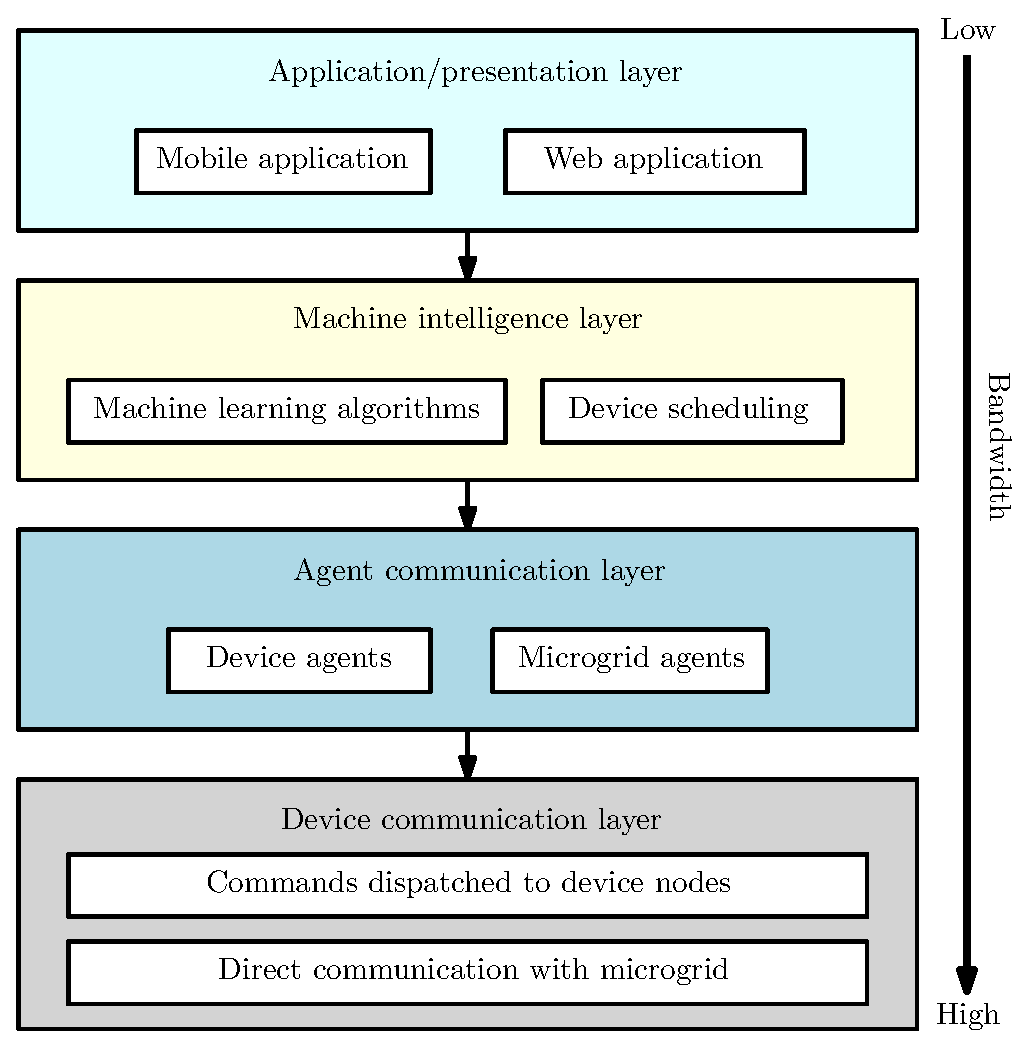
\includegraphics[scale=0.35]{../figs/ipe/BEMS-softwareArchitecture}
  \end{figure}
\end{frame}

\begin{frame}{Introduction}{}
  % applications of mobile robot navigation and problem description
  \begin{figure}
  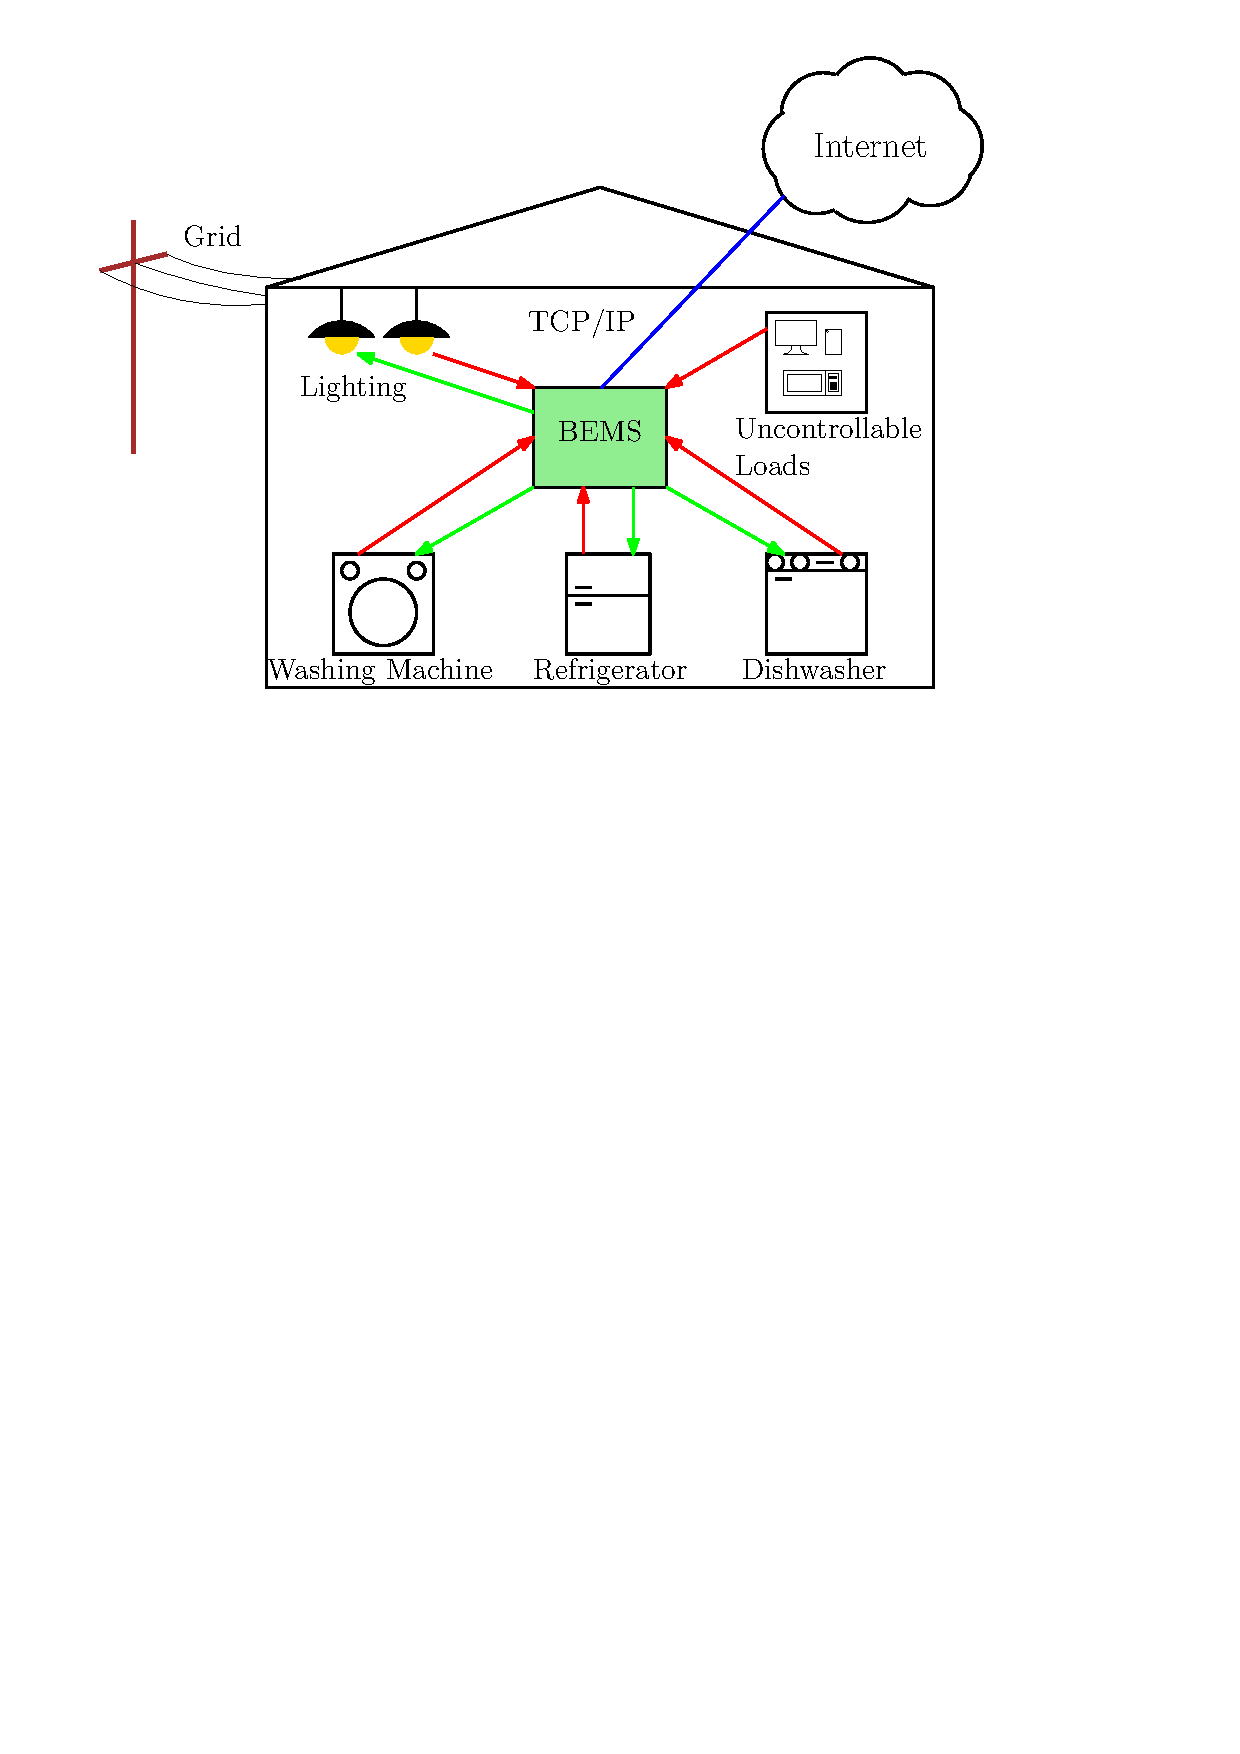
\includegraphics[scale=0.45]{../figs/ipe/bemsdiagram}
  \end{figure}
\end{frame}

\section{Progress}
\begin{frame}{Progress}{}
	\begin{itemize}
		\item Solved communication issue between the Flask webserver and the ControlAgent
		\item Implemented communication between the platform and the WeMo Switch (toggling On and Off)
		\item Queried device for power, energy consumption
	\end{itemize}
\end{frame}

\begin{frame}{Progress}{}
	\begin{itemize}
		\item Changed publish/subscribe messaging system 
		\item Delimited \texttt{topic} and \texttt{method}, \texttt{args} with " " while \texttt{method} and \texttt{args} are delimited with a forward slash
		\item Format: \texttt{topic method/args}
		\item Python \texttt{str.split} method can be used for parsing this string
		\item Exceptions are still being thrown by ZMQ when the button is toggled quickly
		\item \texttt{try}, \texttt{except} statement to handle the exception
	\end{itemize}
\end{frame}

\begin{frame}{Progress}{}
	\begin{figure}
		\centering
		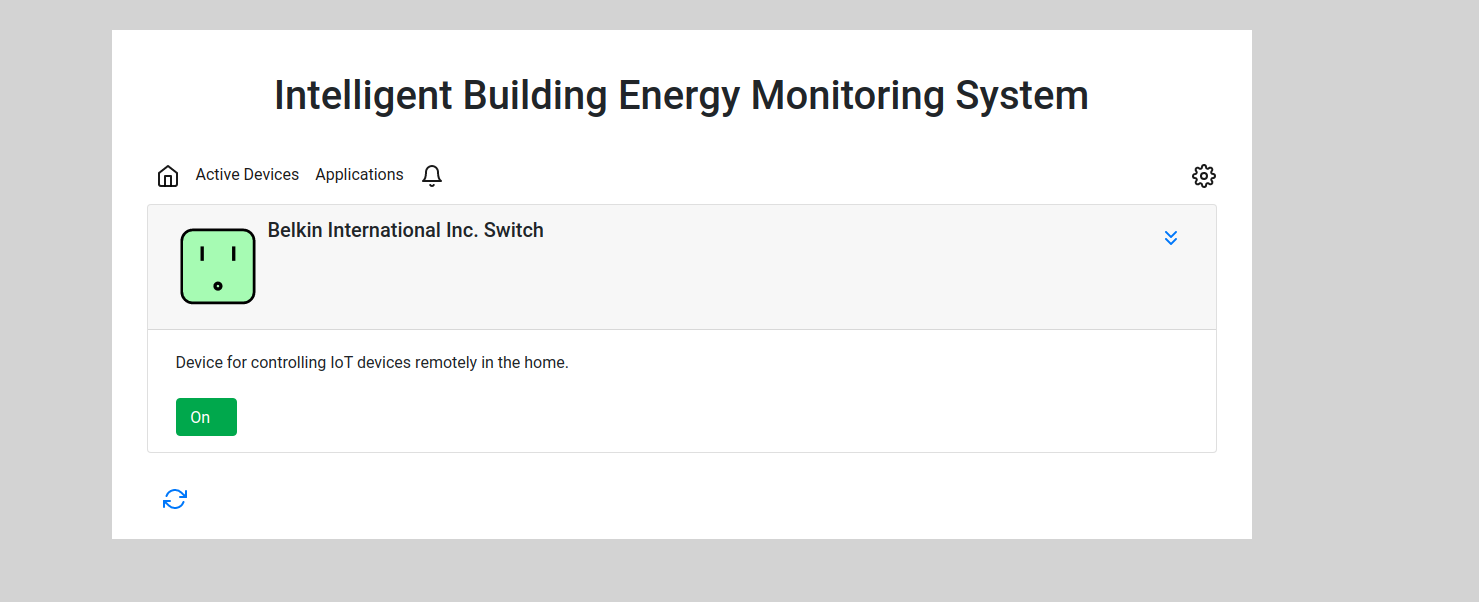
\includegraphics[scale=0.2]{../figs/img/activeDevices2020-07-23.png}
		\caption{Belkin Switch listing in active devices page}
	\end{figure}
\end{frame}

\begin{frame}{Progress}{}
	\begin{itemize}
		\item Implemented in the \texttt{getState} method in the \texttt{WeMoAPI} to query the device for \texttt{InsightParams}
		\item 		\[8 \vert 1595533155 \vert 278 \vert 0 \vert 2829 \vert 1209600 \vert 29 \vert 1745 
		\vert 73977 \vert 1201816.000000 \vert 8000
		\] 
		\item Connected to RPi
	\end{itemize}
\end{frame}

\begin{frame}{Progress}{}
\begin{itemize}
\item State
\item Seconds of last state change
\item Last on seconds
\item Seconds on today
\item Unknown
\item Total seconds
\item Unknown
\item Power(mW)
\item Energy used today (mW*min)
\item Energy used total (mW*min)
\item Unknown
\end{itemize}
\end{frame}


\section{Plans}
\begin{frame}{Plans}{}
\begin{itemize}
	\item Redraw the high-level architecture figure with hand-drawn figures to reduce file size
	\item Continue working on adding the power consumption to the UI 
	\item Once finished with the Switch, work on adding the motor API
\end{itemize}
\end{frame}
\begin{frame}
\Huge
\center
Any Questions?
\end{frame}
\end{document}


%%% Local Variables:
%%% mode: latex
%%% TeX-master: "../progressPresMain"
%%% End:
